  \begin{center}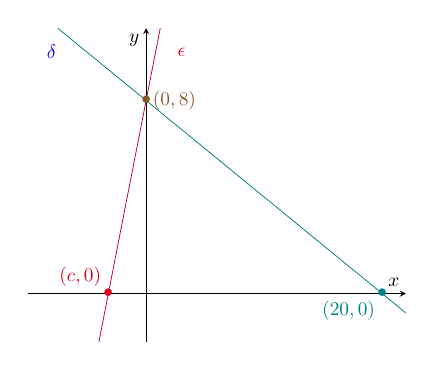
\begin{tikzpicture}[scale=0.7]\begin{axis}[xmin=-10, xmax=22, ymin=-2, ymax=11, axis lines=center, xtick=\empty, ytick=\empty,]
\addplot[purple,domain=-6:3,samples=15]{2.5*x+8};
\addplot[blue!50!green, domain=-10:22,samples=15]{-.4*x+8};
\draw(axis cs: -8, 10)node[blue]{$\delta$}(axis cs: 3, 10)node[purple!50!red]{$\epsilon$};
\draw[brown!70!black](axis cs: 0,8)node{$\bullet$}node[anchor=west]{$(0,8)$};
\draw[blue!50!green,thick](axis cs: 20,0)node{$\bullet$}node[anchor=north east]{$(20,0)$};
\draw[purple!50!red,thick](axis cs: -3.2,0)node{$\bullet$}node[anchor=south east]{$(c,0)$};
\draw(axis cs:0, 10.5)node[anchor=east]{$y$}(axis cs: 21,0)node[anchor=south]{$x$};
\end{axis}\end{tikzpicture}\end{center}
In the $xy$-plane above, line $\delta$ is perpendicular to line $\epsilon$ when the $x$ and $y$ axes are using the same scale.  In the diagram the $x$ and $y$ axes are scaled differently.  What is the value of $c$?\\


\ifsat
	\begin{enumerate}[label=\Alph*)]
		\item $-\frac{2}{5} $ 
		\item $-\frac{16}{5} $ % 
		\item $-\frac{5}{2} $
		\item $\frac{5}{2} $ 
	\end{enumerate}
\else
\fi

\ifacteven
	\begin{enumerate}[label=\textbf{\Alph*.},itemsep=\fill,align=left]
		\setcounter{enumii}{5}
		\item $-\frac{2}{5} $ 
		\item $-\frac{16}{5} $ % 
		\item $-\frac{5}{2} $
		\addtocounter{enumii}{1}
		\item $\frac{5}{2} $ 
		\item None of these. 
	\end{enumerate}
\else
\fi

\ifactodd
	\begin{enumerate}[label=\textbf{\Alph*.},itemsep=\fill,align=left]
		\item $-\frac{2}{5} $ 
		\item $-\frac{16}{5} $ % 
		\item $-\frac{5}{2} $
		\item $\frac{5}{2} $ 
		\item None of these. 
	\end{enumerate}
\else
\fi

\ifgridin
 $-\frac{16}{5} $ % 
		
\else
\fi

